% !TeX root = surprises.tex

\selectlanguage{hebrew}

\chapter{בניית מצולע משוכלל עם 
$17$
צלעות}
\label{c.heptadecagon}

%%%%%%%%%%%%%%%%%%%%%%%%%%%%%%%%%%%%%%%%%%%%%%%%%%%%%%%%%%%

היוונים ידעו לבנות רק ארבעה מצולעים משוכללים: המשולש, הריבוע, המחומש והמצולע המשוכלל עם 
$15$
צלעות. בנוסף, נתון מצולע משוכלל עם
$n$
צלעות, ניתן לבנות מצולע משוכלל עם
$2n$
על ידי בניית המעגל החוסם ובניית חוצה הזווית המרכזית (איור%
~\ref{f.hept-double}).
לא היתה שום התקדמות עד
$1796$
כאשר
\L{Carl Friedrich Gauss}
התעורר בוקר אחד, מעט לפני יום הולדתו ה-%
$19$,
ועל ידי "חשיבה מרוכזת" מצא דרך לבנות 
\L{heptadecagon},
מצולע משוכלל עם
$17$
צלעות. הישג זה שיכנע אותו להיות מתמטיקאי.

סעיף%
~\ref{s.hept-regular}
דן בקשר בין צלע של מצולע החסום על ידי מעגל לבין הזווית המרכזית שעליה הוא נשען. סעיף%
~\ref{s.fundamental}
מביא ללא הוכחה את המשפט הבסיסי של אלגברה. סעיף%
~\ref{s.roots}
מציג את שורשי היחידה, השורשים של הפולינום
$x^n-1$,
שעומדים במרכז ההוכחה של
\L{Gauss}.
סעיפים%
~\ref{s.gauss}
ו-%
~\ref{s.derivation}
מביאים את הוכחה של
\L{Gauss}
שמבוססת על סמטריות של פולינומים.
\L{Gauss}
פיתח נוסחה שה-%
\L{heptadecagon}
בן-בנייה, אבל בנייה גיאומטריה לא פורסמה במשך כמעט מאה שנה. סעיף%
~\ref{s.construction}
מביא בנייה אלגנטית של
\L{James J. Callagy}.
סעיף%
~\ref{s.hept-pentagon}
מראה איך ניתן לפתח בניות של מחומש משוכלל גם באמצעות גיאומטריה וגם באמצעות טריגונומטריה.

ההוכחה ישירה יותר אם מציגים אותה עם מספרים מרוכבים. חומר זה מופרד במסגרות וניתן לדלג עליו.
\begin{figure}[tb]
\begin{center}
\begin{tikzpicture}[scale=.4]
\coordinate (O) at (0,0);
\vertex{O};
\foreach \x/\name/\n/\po in {0/a/A/right,1/b/B/above,2/c/C/left,3/d/D/below left,4/e/E/below right} {
  \coordinate (\name) at ($(O)+(\x*72+18:3cm)$);
}
\draw (a) -- (b) -- (c) -- (d) -- (e) -- (a);
\node[draw,circle through=(a)] at (O) {};
\draw (d) -- (O) -- (e);
\draw [very thick,dotted] (O) -- (-90:3) -- (e) -- (-90:3) -- (d);
\end{tikzpicture}
\end{center}
\caption{בניית מצולע משוכלל עם $10$ צלעות ממחומש משוכלל}\label{f.hept-double}
\end{figure}

\section{בנייה של מצולעים משוכללים}\label{s.hept-regular}

הבנייה של 
\L{heptadecagon}
היתה אבן דרך להוכחת משפט
\L{Gauss-Wantzel}:
מצולע משוכלל עם 
$n$
צלעות הוא בן-בנייה עם סרגל ומחוגה אם ורק אם 
$n$
הוא מכפלה של חזקה של
$2$
ואפס או יותר מספרי 
\L{Fermat}
ראשונים
\textbf{שונים}
$2^{2^k}+1$.
מספרי 
\L{Fermat}
הראשוניים הידועים הם:
\[
F_0=3,\: F_1=5,\: F_2=17,\: F_3=257,\: F_4=65537\,.
\]
מצולע משוכלל עם
$257$
צלעות נבנה לראשונה על ידי
\L{Magnus Georg Paucker}
ב-%
$1822$
ועל ידי
\L{Friedrich Julius Richelot}
ב-%
$1832$.
ב-%
$1894$
\L{Johann Gustav Hermes}
טען שבנה מצולע משוכלל עם
$65537$
צלעות.
כתב היד שלו נשמר באוניברסיטת 
\L{G\"{o}ttigen}.

כדי לבנות מצולע משוכלל מספיק לבנות קטע קו באורך 
$\cos \theta$,
כאשר
$\theta$ 
היא הזווית המרכזית במעגל היחידה הנתמך על ידי המיתר שהוא צלע של המצולע. נתון קטע הקו
$\overline{OB}=\cos\theta$,
בנו אנך ב-%
$B$
וסמנו את החיתוך שלו עם מעגל היחידה ב-%
$C$.
אזי:
\begin{eqn}
\overline{OC}&=&1\\
\cos \theta&=&\disfrac{\overline{OB}}{\overline{OC}}=\overline{OB}\,.
\end{eqn}
המיתר 
$\overline{AC}$
הוא צלע של המצולע (איור%
~\ref{f.hept-central1}).

\begin{figure}[tb]
\begin{center}
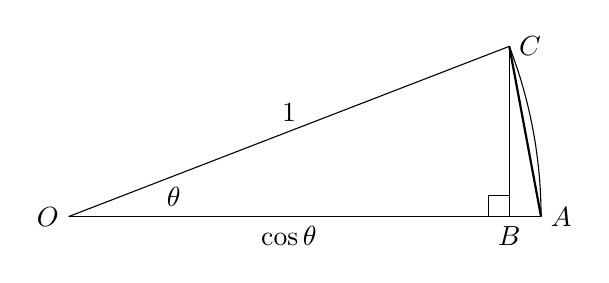
\begin{tikzpicture}[scale=1.5]
\coordinate (O) at (0,0) node[left] {$O$} node[above right,xshift=32pt] {$\theta$};
\coordinate (A) at (4,0);
\node[right] at (A) {$A$};
\draw (O) -- (A);
\draw (A) arc(0:21.12:4);
\coordinate (C) at (21.12:4cm);
\draw (O) -- node[above] {$1$} (C);
\node[right] at (C) {$C$};
\draw (C) -- (C |- A) coordinate (B);
\node[below] at (B) {$B$};
\draw[rotate=90] (B) rectangle +(5pt,5pt);
\draw[thick] (A) -- (C);
\path (O) -- node[below] {$\cos \theta$} (B); 
\end{tikzpicture}
\caption{הקוסינוס של הזווית המרכזית של מצולע משוכלל}
\label{f.hept-central1}
\end{center}
\end{figure}
נתון קטע קו שאורכו מוגדר כ-%
$1$,
האורכים שניתנים לבנייה הם אלה שניתן לקבל מאורכים קיימים תוך שימוש בפעולות 
$\{+,-,\times,/,\surd\}$ 
(סעיף%
~\ref{s.trisect-constructible}).
\L{Gauss}
הראה ש-%
$\cos(360^\circ/17$, 
הקוסינוס של הזווית המרכזית של 
\L{heptadecagon},
בן-בנייה כי ניתן לבטא אותו תוך שימוש רק בפעולות הללו:
\begin{eqn}
\cos\left(\disfrac{2\pi}{17}\right) &=& 
-\disfrac{1}{16}+\disfrac{1}{16}\sqrt{17} + 
     \disfrac{1}{16}\sqrt{34-2\sqrt{17}}
    + \\
    &&
     \disfrac{1}{8}\sqrt{
     17+3\sqrt{17} - 
     \sqrt{34-2\sqrt{17}}
   -2
     \sqrt{34+2\sqrt{17}}
   }\,.
\end{eqn}

%%%%%%%%%%%%%%%%%%%%%%%%%%%%%%%%%%%%%%%%%%%%%%%%%%%%%%

\section{המשפט הבסיסי של אלגברה}\label{s.fundamental}

נשתמש במשפט שלהלן ללא הוכחה.

\begin{theorem}\label{thm.fundamental}
לכל פולינום ממעלה 
$n$
בדיוק 
$n$
שורשים.
\end{theorem}
הבאתי ניסוח פשוט של המשפט כי כל מה שאנחנו חייבים לדעת הוא קיימים
$n$
שורשים.

\begin{advanced}
\textbf{המשפט הבסיסי של אלגברה (\L{The Fundamental Theorem of Algebra})}
טוען שלכל פולינום לא-קבוע ממעלה 
$n$
במשתנה אחד עם מקדמים מרוכבים יש בדיוק 
$n$
שורשים מרוכבים. אם קיימים מספר שורשים בעלי אותו ערך, עלינו לספור את כולן. ל:
\[
x^2-4x+4=(x-2)(x-2)
\]
שני שורשים שערכם
$2$.
לפולינום 
$x^2+1$
עם מקדמים שלמים יש שני שורשים מרוכבים
$\pm\sqrt{-1}$.
באופן משונה, למרות שנושא המשפט קשור למבנים אלגבריים סופיים (פולינומים ממעלה
$n$
עם
$n$
שורשים), כדי להוכיח את המשפט חייבים להשתמש בשיטות מאנליזה, בדרך כלל, אנליזה של מספרים מרוכבים.
\end{advanced}

%%%%%%%%%%%%%%%%%%%%%%%%%%%%%%%%%%%%%%%%%%%%%%%%%%%%%%

\section{שורשי היחידה}\label{s.roots}

לפי המשפט בסיסי של אלגברה (משפט~%
\ref{thm.fundamental})
לפולינום
$x^{n}-1=0$
יש 
$n$
שורשים עבור כל מספר שלם
$n>	 1$.
שורש אחד הוא
$x=1$
ולכן קיימים
$n-1$
שורשים נוספים. נסמן שורש אחד מתוכם ב-%
$r$.
בגלל ש-%
$r^{n}=1$,
$r$
נקרא שורש היחידה מסדר
$n$.
מה עם
$r^2$?
\[
(r^2)^n=(r^{n})^2=1^2=1\,.
\]
חישוב דומה מראה ש-%
$n$
המספרים:
\[
1, r, r^2, \ldots, r^{n-2}, r^{n-1}
\]
הם שורשים של היחידה מסדר
$n$.
\begin{advanced}
יהי
$r=\cos \left(\frac{2\pi}{n}\right) + i\sin  \left(\frac{2\pi}{n}\right)$.
לפי הנוסחה של
\L{de Moivre}:
\[
\left[\cos \left(\frac{2\pi}{n}\right) + i\sin  \left(\frac{2\pi}{n}\right)\right]^{n}=
\cos \left(\frac{2 n\pi}{n}\right) + i\sin  \left(\frac{2 n\pi}{n}\right)= 1\,.
\]
\vspace{-2ex}
\end{advanced}

\begin{theorem}\label{thm.roots-of-unity}
יהי
$n$
מספר ראשוני ו-%
$r$
שורש היחידה מסדר 
$n$.
אזי:
\[
\{1,r,r^2,\ldots,r^{n-2},r^{n-1}\}
\]
שונים זה מזה ולכן הם מהווים את כל שורשי היחידה מסדר
$n$.
\end{theorem}

\begin{proof}
נניח שהשורשים לא שונים כך ש-%
$r^i=r^j$
עבור שני מספרים
$1\leq i<j\leq n$.
אזי
$r^j/r^i=r^{j-i}=1$,
כלומר, קיים לפחות מספר שלם חיובי אחד 
$i'$
פחות מ-%
$n$
כך ש-%
$r^{i'}=1$.
יהי
$m$
המספר השלם החיובי הקטן ביותר. לפי אלגוריתם החילוק של שלמים,
$n=ml+k$
עבור
$0<l<n$,
$0\leq k<m$.
מ:
\[
1=r^n=r^{ml+k}=(r^m)^l\cdot r^k=1^l\cdot r^k=r^k\,,
\]
מתקבל
$0\leq k<m$ 
ו-%
$r^k=1$.
אבל
$m$
הוא המספר השלם החיובי הקטן ביותר המקיים את התנאי, חייב להתקיים 
$k=0$
ו-%
$n=ml$
סתירה להנחה ש-%
$n$
ראשוני.
\end{proof}
\begin{theorem}
יהי
$\{a_1,a_2,\ldots,a_{n-1},a_n\}$
השורשים של פולינום
$f(x)$
מסדר
$n$.
אזי:
\begin{equation}\label{eq.viete}
f(x) =(x-a_1) (x-a_2)\cdots (x-a_{n-1})(x-a_n)\,.
\end{equation}
\end{theorem}

\begin{proof}

לפי ההגדרה אם
$a_i$
הוא שורש של
$f(x)$
אזי
$f(a_i)=0$,
ולכן:
\begin{eqn}
f(a_i)&=&(a_i-a_1) (a_i-a_2)\cdots (a_i-a_{n-1})(a_i-a_n)\\
&=&\cdots (a_i-a_i) \cdots =0\,.
\end{eqn}
מכאן ש-%
$f(x)=(x-a_i)g_i(x)$
עבור 
$g_i(x)$
כלשהו ובאינדוקציה הדבר נכון לכל השורשים.
\end{proof}
ממשוואה%
~\ref{eq.viete}
קל לראות שהמקדם של
$x^n-1$
הוא:
\[
-(a_1+a_2+\cdots+a_{n-1}+a_n)\,.
\]
אבל המקדם של
$x^n-1$
עבור
$n\geq0$
הוא אפס ולכן:
\begin{eqn}
1+r+r^2+\cdots + r^{n-2}+r^{n-1}&=&0\\
r+r^2+\cdots + r^{n-2}+r^{n-1}&=&-1\,.
\end{eqn}
עבור
\L{heptadecagon}
המשוואה היא:
\begin{eqnlabels}\label{eq.minus-one}
&&\nonumber{}r+r^2+r^3+r^4+r^5+r^6+r^7+r^8+\\
&&\qquad r^9+r^{10}+r^{11}+r^{12}+r^{13}+r^{14} + r^{15}+r^{16}=-1\,.\end{eqnlabels}

%%%%%%%%%%%%%%%%%%%%%%%%%%%%%%%%%%%%%%%%%%%%%%%%%%%%%%%%

\section{ההוכחה של 
\L{Gauss}
שניתן לבנות 
\L{heptadecagon}}\label{s.gauss}

\L{Gauss}
הבין שאין חובה לעבוד עם השורשים בסדר הטבעי שלהם
$r,r^2,\ldots,r^{16}$. 
החזקות של
$r^3$
נותנות את כל השורשים אבל בסדר שונה:
\[
\renewcommand{\arraystretch}{1.1}
\begin{array}{l}
r^1, \;r^{1\cdot 3 =3},\; r^{3\cdot 3=9},\; r^{9\cdot 3=27=10},\; r^{10\cdot 3=30=13},\; r^{13\cdot 3=39=5},\; r^{5\cdot 3=15},\\ r^{15\cdot 3=45=11},
r^{11\cdot 3 =33=16}, \;r^{16\cdot 3=48=14},\; r^{14\cdot 3=42=8},\; r^{8\cdot 3=24=7},\\r^{7\cdot 3=21=4},\; r^{4\cdot 3=12},\; r^{12\cdot 3=36=2},\; r^{2\cdot 3=6}\,,
\end{array}
\]
כאשר צמצמנו את השורשים מודולו
$17$:
\[
r^{17m+k}=(r^{17})^m\cdot r^k=1^m\cdot r^k=r^k\,.
\]
חשוב שתבדקו שהרשימה כוללת את כל השורשים  (פרט ל-%
$1$)
בדיוק פעם אחת:
\begin{equation}\label{eq.roots}
r^1, r^3, r^9, r^{10}, r^{13}, r^5, r^{15}, r^{11}, r^{16}, r^{14}, r^8, r^7, r^4, r^{12}, r^2, r^6\,.
\end{equation}

נתון פולינום ריבועי מונית שהשורשיו הם:
$a,b$:
\[
y^2+yx+q=(y-a)(y-b)=0\,,
\]
ניתן לחשב את המקדמים
$p,	q$
מהשורשים
(פרק%
\ref{c.quadratic}):
\[
p=-(a+b)\,,\quad q=ab\,.
\]
לכן אם ניתן 
$a+b$
ו-%
$ab$
נוכל לכתוב את המשוואה הריבועית בשורשיו הם
$a,b$.

יהי
$a_0$
סכום השורשים במקומות האי-זוגיים במשוואה%
~\ref{eq.roots}:
\[
a_0=r + r^9 + r^{13} +r^{15} +r^{16} + r^8+r^4+r^2\,,
\]
ויהי
$a_1$
סכום השורשים במקומות הזוגיים במשוואה%
~\ref{eq.roots}:
\[
a_1=r^3 + r^{10} + r^{5} +r^{11} +r^{14} + r^7+r^{12}+r^6\,.
\]
כדי לקבל את
$a_0,a_1$
כשורשים של משוואה ריבועית, תחילה נחשב את הסכום שלהם:
\[
a_0+a_1=r + r^2 + \cdots +r^{16}=-1\,.
\]
כדי למצוא את המשוואה הריבועית עלינו לחשב את
$a_0a_1$.
החישוב מעט מסורבל ומוצג באיור%
~\ref{fig.a0a1}.
הערכים של
$r^ir^j$
רשומים לאחר חישוב
$r^{(i+j) \bmod 17}$.
מתחת לכל שורש נמצא מספר המופעים שלו עד כה. בדקו שכל שורש מופיע בדיוק ארבע פעמיים כך שערכה של המכפלה הוא 
$-4$.
\begin{figure}[tb]
\begin{eqn}
a_0a_1&=&(r + r^9 + r^{13} +r^{15} +r^{16} + r^8+r^4+r^2)\;\cdot\\
&&(r^3 + r^{10} + r^{5} +r^{11} +r^{14} + r^7+r^{12}+r^6)\\
&=&\occ{4}{1} + \occ{11}{1} + \occ{6}{1} + \occ{12}{1} + \occ{15}{1} + \occ{8}{1} + \occ{13}{1} + \occ{7}{1} +\\
&&\occ{12}{2} + \occ{2}{1} + \occ{14}{1} + \occ{3}{1} + \occ{6}{2} + \occ{16}{1} + \occ{4}{2} + \occ{15}{2} +\\
&&\occ{16}{2} + \occ{6}{3} + \occ{1}{1} + \occ{7}{2} + \occ{10}{1} + \occ{3}{2} + \occ{8}{2} + \occ{2}{2}\;\;\: +\\
&&\occ{1}{2} + \occ{8}{3} + \occ{3}{3} + \occ{9}{1} + \occ{12}{3} + \occ{5}{1} + \occ{10}{2} + \occ{4}{3}\;\;\: +\\
&&\occ{2}{3} + \occ{9}{2} + \occ{4}{4} + \occ{10}{3} + \occ{13}{2} + \occ{6}{4} + \occ{11}{2} + \occ{5}{2} \:+\\
&&\occ{11}{3} + \occ{1}{3} + \occ{13}{3} + \occ{2}{4} + \occ{5}{2} + \occ{15}{3} + \occ{3}{4} + \occ{14}{2} \;+\\
&&\occ{7}{3} + \occ{14}{3} + \occ{9}{3} + \occ{15}{4} + \occ{1}{4} + \occ{11}{4} + \occ{16}{3} + \occ{10}{4} +\\
&&\occ{5}{4} + \occ{12}{4} + \occ{7}{4} + \occ{13}{4} + \occ{16}{4} + \occ{9}{4} + \occ{14}{4} + \occ{8}{4}\\
&=&-4\,.
\end{eqn}
\selectlanguage{hebrew}
\caption{החישוב של $a_0a_1$}\label{fig.a0a1}
\end{figure}

מ-%
$a_0\!+\!a_1\!=\!-1$
ו-%
$a_0a_1\!=\!-4$,
אנו יודעים ש-%
$a_0,a_1$
הם השורשים של המשוואה:
\[
x^2+x-4=0
\]
ששורשיו הם:
\[
a_{0,1} = \frac{-1\pm\sqrt{17}}{2}\,.
\]
יהי
$b_0,b_1,b_2,b_3$
הסכום של כל שורש רביעי החל מ-%
$r^1,r^3,r^9,r^{10}$,
בהתאמה:
\begin{eqn}
b_0&=& r^1+ r^{13} + r^{16} + r^4\\
b_1&=& r^3+ r^{5} + r^{14} + r^{12}\\
b_2&=& r^9+ r^{15} + r^{8} + r^2\\
b_3&=& r^{10}+ r^{11} + r^{7} + r^6\,.
\end{eqn}
בדקו ש-%
$b_0+b_2=a_0, b_1+b_3=a_1$
וחשבו את המכפלות המתאימות:
\begin{eqn}
b_0b_2&=&(r + r^{13} + r^{16} +r^4)\;\times\\
&&(r^9 + r^{15} + r^{8} +r^{2})\\
&=& r^{10}+r^{16}+r^9+r^3+\\
&& r^{5}+r^{11}+r^4+r^{15}+\\
&& r^{8}+r^{14}+r^7+r^1\;\:+\\
&& r^{13}+r^{2}+r^{12}+r^6\\
&=&-1\,.
\end{eqn}
\begin{eqn}
b_1b_3&=&(r^3 + r^{5} + r^{14} +r^{12})\times\\
&&(r^{10} + r^{11} + r^{7} +r^{6})\\
&=& r^{13}+r^{14}+r^{10}+r^9\;+\\
&& r^{15}+r^{16}+r^{12}+r^{11}+\\
&& r^{7}+r^{8}+r^4+r^3\quad\;\;+\\
&& r^{5}+r^{6}+r^{2}+r^1\\
&=&-1\,.
\end{eqn}
נסכם את החישובים:
\begin{eqn}
b_0+b_2&=&a_0\\
b_0b_2&=&-1\\
b_1+b_3&=&a_1\\
b_1b_3&=&-1\,.
\end{eqn}
$b_0,b_2$ 
הם שורשיו של
$y^2-a_0y-1= 0$
ו-%
$b_1,b_3$
הם שורשיו של
$y^2-a_1y-1 =0$.
מהערכים שחישבנו קודם עבור 
$a_0,a_1$,
מתקבלים השורשים
$b_0,b_1$
(איור~%
\ref{fig.b0b1}).

\begin{figure}[tb]
\begin{eqn}
b_0&=&\disfrac{a_0+\sqrt{a_0^2+4}}{2}\\
&=&\disfrac{
     \disfrac{(-1+\sqrt{17})}{2} + 
     \sqrt{\left[\disfrac{(-1+\sqrt{17})}{2}\right]^2+4}
   }{2}\\
&=&\disfrac{
     (-1+\sqrt{17}) + 
     \sqrt{\left[-1+\sqrt{17}\right]^2+16}
   }{4}\\
&=&\disfrac{
     (-1+\sqrt{17}) + 
     \sqrt{34-2\sqrt{17}}
   }{4}\\
b_1&=&\disfrac{a_1+\sqrt{a_1^2+4}}{2}\\
&=&\disfrac{
     \disfrac{(-1-\sqrt{17})}{2} + 
     \sqrt{\left[\disfrac{(-1-\sqrt{17})}{2}\right]^2+4}
   }{2}\\
&=&\disfrac{
     (-1-\sqrt{17}) + 
     \sqrt{\left[-1-\sqrt{17}\right]^2+16}
   }{4}\\
&=&\disfrac{
     (-1-\sqrt{17}) + 
     \sqrt{34+2\sqrt{17}}
   }{4}\,.
\end{eqn}
\selectlanguage{hebrew}
\caption{החישוב של $b_0,b_1$}\label{fig.b0b1}
\end{figure}
לבסוף יהי
$c_0,c_4$ 
הסכום של כל שורש שמיני החל מ-%
$r^1,r^{13}$,
בהתאמה:
\begin{eqn}
c_0&=&r^1+r^{16}\\
c_4&=&r^{13}+r^4\\
c_0+c_4&=&r^1+r^{16}+r^{13}+r^4=b_0\\
c_0c_4&=&(r^1+r^{16})\cdot(r^{13}+r^4)\\
&=&r^{14}+r^5+r^{12}+r^3=b_1\,.
\end{eqn}
$c_0,c_4$
הם השורשים של
$y^2-b_0y+b_1=0$.
בגלל ש-%
$\cos(360^\circ/17) = c_0/2$
(איור%
~\ref{f.hept-cosine})
מספיק לחשב את השורש
$c_0=r^1+r^{16}$
(איור%
~\ref{fig.c0}).

\begin{figure}[tb]
\begin{center}

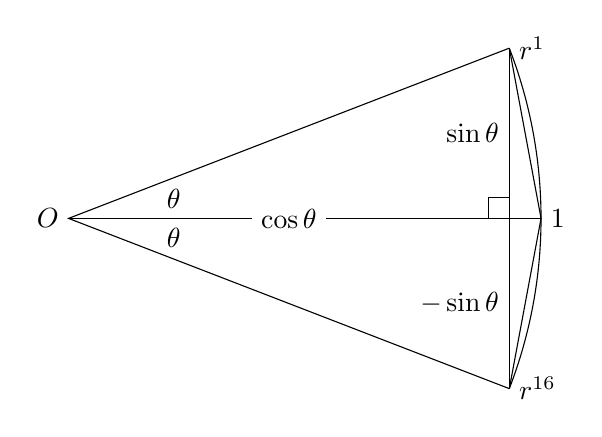
\begin{tikzpicture}[scale=1.5]
\coordinate (O) at (0,0) node[left] {$O$} node[above right,xshift=32pt] {$\theta$} node[below right,xshift=32pt] {$\theta$};
\coordinate (A) at (4,0);
\node[right] at (A) {$1$};
\draw (O) -- (A);
\coordinate (C) at (21.12:4cm);
\coordinate (D) at (-21.12:4cm);
\draw (D) arc(-21.12:21.12:4);
\draw (D) -- (O) -- (C);
\node[right] at (C) {$r^1$};
\node[right] at (D) {$r^{16}$};
\draw (C) -- (C |- A) coordinate (B);
\draw (D) -- (D |- A);
%\node[below left] at (B) {$B$};
\draw[rotate=90] (B) rectangle +(5pt,5pt);
\draw (D) -- node[left,xshift=-6pt] {$-\sin\theta$} (A) -- node[left,xshift=-6pt] {$\sin \theta$} (C);
\path (O) -- node[fill=white] {$\cos \theta$} (B);
\end{tikzpicture}
\caption{בניית צלע מהזווית המרכזית שהוא כולא}\label{f.hept-cosine}
\end{center}
\end{figure}
\begin{figure}
\begin{eqn}
c_0&=&\disfrac{b_0+\sqrt{b_0^2-4b_1}}{2}\\
&=&\disfrac{
     \disfrac{
     (-1+\sqrt{17}) +
     \sqrt{34-2\sqrt{17}}
   }{4}}{2} + \\
&& 
    \disfrac{
       \sqrt{\left[\disfrac{
     (-1+\sqrt{17}) + 
     \sqrt{34-2\sqrt{17}}
   }{4}\right]^2-4\left[\disfrac{
     (-1-\sqrt{17}) + 
     \sqrt{34+2\sqrt{17}}
   }{4}\right]}
   }{2}\\
&=&-\disfrac{1}{8}+\disfrac{1}{8}\sqrt{17} + 
     \disfrac{1}{8}\sqrt{34-2\sqrt{17}}
    + \\
   &&
     \disfrac{1}{8}\sqrt{
     \left[
     (-1+\sqrt{17}) + 
     \sqrt{34-2\sqrt{17}}
   \right]^2-16\left[
     (-1-\sqrt{17}) + 
     \sqrt{34+2\sqrt{17}}
   \right]}
\\
&=&-\disfrac{1}{8}+\disfrac{1}{8}\sqrt{17} + 
     \disfrac{1}{8}\sqrt{34-2\sqrt{17}}
    + \\
   &&
     \disfrac{1}{8}\sqrt{
     (-1+\sqrt{17})^2 + 
     2(-1+\sqrt{17})\sqrt{34-2\sqrt{17}}+
     (34-2\sqrt{17})
   -}\\
   &&\overline{
     \left[(-16-16\sqrt{17}) + 
     16\sqrt{34+2\sqrt{17}}\right]
   }
\\
&=&-\disfrac{1}{8}+\disfrac{1}{8}\sqrt{17} + 
     \disfrac{1}{8}\sqrt{34-2\sqrt{17}}
    + \\
   &&
     \disfrac{1}{8}\sqrt{
     68+12\sqrt{17} + 
     2(-1+\sqrt{17})\sqrt{34-2\sqrt{17}}
   -16
     \sqrt{34+2\sqrt{17}}
   }
\end{eqn}
\selectlanguage{hebrew}
\caption{החישוב של $c_0$}\label{fig.c0}
\end{figure}
הקוסינוס של הזווית המרכזית של
\L{heptadecagon}
בן-בנייה עם סרגל ומחוגה כי הוא מורכב רק ממספרים רציונליים והפעולות
$\{+,-,\times,/,\surd\}$:
\begin{eqnlabels}
\nonumber{}&&\cos\left(\frac{360^\circ}{17}\right) = 
\frac{c_0}{2}=\\
\nonumber{}&&\qquad{}-\frac{1}{16}+\frac{1}{16}\sqrt{17} + 
     \frac{1}{16}\sqrt{34-2\sqrt{17}}\; +\\
&& \qquad\frac{1}{16}\sqrt{
     68+12\sqrt{17} + 
     2(-1+\sqrt{17})\sqrt{34-2\sqrt{17}}
   -16
     \sqrt{34+2\sqrt{17}}
   }\,.\label{eq.not-gauss}
\end{eqnlabels}

\begin{advanced}
\vspace{-3ex}
\begin{eqn}
r_1+r_{16}&=&\cos\left(\frac{2\pi}{17}\right)+i\sin\left(\frac{2\pi}{17}\right)+\cos\left(\frac{2\cdot 16\pi}{17}\right)+i\sin\left(\frac{2\cdot 16\pi}{17}\right)\\
&=&\cos\left(\frac{2\pi}{17}\right)+i\sin\left(\frac{2\pi}{17}\right)+\cos\left(\frac{-2\pi}{17}\right)+i\sin\left(\frac{-2\pi}{17}\right)\\
&=&2\cos\left(\frac{2\pi}{17}\right)\,.
\end{eqn}
\vspace{-3ex}
\end{advanced}

%%%%%%%%%%%%%%%%%%%%%%%%%%%%%%%%%%%%

\section{פיתוח הנוסחה של %
\L{Gauss}%
}\label{s.derivation}

הנוסחה שקיבלנו עבור 
$\cos (360^\circ/17)$
איננה הנוסחה שניתנה על ידי
\L{Gauss}.
להלן פיתוח של הנוסחה של
\L{Gauss}.

נפשט את
$2(-1+\sqrt{17})\sqrt{34-2\sqrt{17}}$:

\begin{eqn}
2(-1+\sqrt{17})\sqrt{34-2\sqrt{17}} &=&
-2\sqrt{34-2\sqrt{17}} +2\sqrt{17}\sqrt{34-2\sqrt{17}}+\\
&&4\sqrt{34-2\sqrt{17}}-4\sqrt{34-2\sqrt{17}}\\
&=&
2\sqrt{34-2\sqrt{17}} +2\sqrt{17}\sqrt{34-2\sqrt{17}}+\\
&&-4\sqrt{34-2\sqrt{17}}\\
%&=&\left(-2\sqrt{34-2\sqrt{17}} +2\sqrt{17}\sqrt{34-2\sqrt{17}}
%+4\sqrt{34-2\sqrt{17}}\right)\\
%&&-4\sqrt{34-2\sqrt{17}}\\
&=&2(1+\sqrt{17})\sqrt{34-2\sqrt{17}}-4\sqrt{34-2\sqrt{17}}\,.
\end{eqn}
נזכור את הגורם
$-4\sqrt{34-2\sqrt{17}}$
ונפשט את הגורם הראשון. נרבע אותו ואז נוציא שורש הריבועי:

\begin{eqn}
2(1+\sqrt{17})\sqrt{34-2\sqrt{17}}&=&
2\sqrt{\left[(1+\sqrt{17})\sqrt{34-2\sqrt{17}}\right]^2}\\
&=&2\sqrt{(18+2\sqrt{17})(34-2\sqrt{17})}\\
&=&2\sqrt{(18\cdot 34-4\cdot17)+\sqrt{17}(2\cdot 34 - 2\cdot 18)}\\
&=&2\cdot 4\sqrt{34+2\sqrt{17}}\,.
\end{eqn}
נציב את הגורמים ונקבל את הנוסחה של
\L{Gauss}:

\begin{eqn}
\cos\left(\disfrac{2\pi}{17}\right) &=& 
-\disfrac{1}{16}+\disfrac{1}{16}\sqrt{17} + 
     \disfrac{1}{16}\sqrt{34-2\sqrt{17}}
    + \\
    &&
     \disfrac{1}{16}\sqrt{
     68+12\sqrt{17} + 
     2\cdot 4\sqrt{34+2\sqrt{17}}-4\sqrt{34-2\sqrt{17}}
   -16
     \sqrt{34+2\sqrt{17}}
   }\\
&=&-\disfrac{1}{16}+\frac{1}{16}\sqrt{17} + 
     \disfrac{1}{16}\sqrt{34-2\sqrt{17}}
    + \\
    &&
     \disfrac{1}{8}\sqrt{
     17+3\sqrt{17} - 
     \sqrt{34-2\sqrt{17}}
   -2
     \sqrt{34+2\sqrt{17}}
   }
\end{eqn}


\section{בניית
\L{heptadecagon}}
\label{s.construction}

בנו מעגל יחידה שמרכזו
$O$,
עם קוטרים ניצבים
$\overline{PQ},\overline{RS}$
(איור%
~\ref{f.hept-construction1}).
בנו נקודה
$A$
כך ש-%
$\overline{OA}=\disfrac{1}{4}\overline{OR}$.

\begin{figure}[tb]
\begin{center}
\begin{tikzpicture}[scale=1.5]
\clip (-5,-1.8) rectangle (5,1.8);

\node at (-.2,1.5) {$\cdots$};
\node at (-.2,1.7) {$R$};
\node at (-.2,-1.5) {$\cdots$};
\node at (-.2,-1.7) {$S$};

\coordinate (O) at (0,0);
\draw (O) circle (4cm);
\coordinate (P) at (4,0);
\coordinate (R) at (0,4);
\coordinate (Q) at (-4,0);
\coordinate (S) at (0,-4);
\coordinate (A) at (0,1);
\coordinate (B) at (.78,0);
\coordinate (C) at (-1.28,0);
\draw (P) -- (Q);
\draw (R) -- (S);
\path (O) -- node[left,xshift=2pt,yshift=-4pt] {\sm{\frac{1}{4}}} (A);
\draw[dashed] (P) -- ($(P)!1.5!(A)$);
\draw (A) -- node[above] {$\frac{\sqrt{17}}{4}$} (P);
\draw (C) -- (A) -- (B);
\foreach \c/\where in {O/below left, P/right, Q/left, R/above, S/below, A/above left, B/below, C/below} {
  \fill (\c) circle(1pt) node[\where] {$\c$};
}
\draw (O) rectangle(+6pt,+6pt);
\node[below right,xshift=8pt,yshift=-4pt] at (A) {\sm{\alpha}};
\node[below right,xshift=-3pt,yshift=-4pt] at (A) {\sm{\alpha}};
\node[below left,xshift=1pt,yshift=-2pt] at (A) {\sm{\beta}};
\node[below left,xshift=-4pt,yshift=4pt] at (A) {\sm{\beta}};
\draw[<->] ($(C)+(0,-16pt)$) -- node[below] {\sm{\frac{1+\sqrt{17}}{16}}} ($(O)+(0,-16pt)$);
\draw[<->] ($(O)+(0,-16pt)$) -- node[below,xshift=4pt] {
\sm{
\frac{-1+\sqrt{17}}{2}
}
} ($(B)+(0,-16pt)$);
\end{tikzpicture}
\caption{בניית \L{heptadecagon} (1)}\label{f.hept-construction1}
\end{center}
\end{figure}
לפי משפט פיתגורס:
\[
\overline{AP}=\sqrt{(1/4)^2+1^2}=\sqrt{17}/4\,.
\]
תהי
$B$
נקודת החיתוך של 
$\angle OAP$
וקטע הקו
$\overline{OP}$,
ותהי 
$C$
נקודת החיתוך של חוצה הזווית המשלימה ל-%
$\angle OAP$ 
וקטע הקו
$\overline{QO}$.
לפי משפט חוצה הזווית הפנימית (משפט%
~\ref{thm.angle-bisector}):
\begin{eqn}
\disfrac{\overline{OB}}{\overline{BP}}&=&\disfrac{\overline{AO}}{\overline{AP}}\\
\disfrac{\overline{OB}}{1-\overline{OB}}&=&\disfrac{1/4}{\sqrt{17}/{4}}\\
\overline{OB}&=&\disfrac{1}{1+\sqrt{17}}=\disfrac{1}{1+\sqrt{17}}\cdot \disfrac{1-\sqrt{17}}{1-\sqrt{17}}\\
&=&\disfrac{-1+\sqrt{17}}{16}\,,
\end{eqn}
ולפי משפט חוצה הזווית החיצונית (משפט%
~\ref{thm.external-angle-bisector}):
\begin{eqn}
\disfrac{\overline{OC}}{\overline{CP}}&=&\disfrac{\overline{AO}}{\overline{AP}}\\
\disfrac{\overline{OC}}{1+\overline{OC}}&=&\disfrac{1/4}{\sqrt{17}/{4}}\\
\overline{OC}&=&\disfrac{1}{-1+\sqrt{17}}=\disfrac{1}{-1+\sqrt{17}}\cdot \disfrac{1+\sqrt{17}}{1+\sqrt{17}}\\
&=&\disfrac{1+\sqrt{17}}{16}\,.
\end{eqn}
בנו
$D$
על
$\overline{OP}$
כך ש-%
$\overline{CD}=\overline{CA}=a$
(איור%
~\ref{f.hept-construction2}).
לפי משפט פיתרורס:
\begin{figure}[tb]
\begin{center}
\begin{tikzpicture}[scale=1.5]
\clip (-5,-1.5) rectangle (5,1.5);
\coordinate (O) at (0,0);
\draw (O) circle (4cm);
\coordinate (P) at (4,0);
\coordinate (R) at (0,4);
\coordinate (Q) at (-4,0);
\coordinate (S) at (0,-4);
\coordinate (A) at (0,1);
\coordinate (B) at (.78,0);
\coordinate (C) at (-1.28,0);

\coordinate (D) at (.344,0);
\coordinate (E) at (2.05,0);
\coordinate (M) at (-1.8275,0);
\coordinate (F) at (0,-1);

\draw (P) -- (Q);
\draw (R) -- (S);
\draw (A) -- (P);
\draw (C) -- node[above] {$a$} (A) -- node[above,xshift=2pt] {$b$} (B);
\path (Q) -- node[below] {$f$}  (M);
\path (B) -- node[below] {$b$} (E);

\path[name path=circ] (M) circle (2.1725cm);
\path[name path=yaxis] (R) -- (S);
\path[name intersections={of=circ and yaxis,by={F1,F}}];
\draw (M) -- node[below] {$f$} (F);

\draw[<->] ($(C)+(0,-15pt)$) -- node[fill=white] {$a$} ($(D)+(0,-15pt)$);

\foreach \c/\where in {O/below left, P/right, Q/left, R/above, S/below, A/above left, B/below, C/below, D/below, E/below, M/below left, F/below left} {
  \fill (\c) circle(1pt) node[\where] {$\c$};
}
\draw (O) rectangle(+6pt,+6pt);
\end{tikzpicture}
\caption{בניית \L{heptadecagon} (2)}\label{f.hept-construction2}

\end{center}
\end{figure}
\begin{eqn}
\overline{CD}=\overline{CA}&=&\sqrt{\overline{OA}^2+\overline{OC}^2}\\
&=&\sqrt{\left(\disfrac{1}{4}\right)^2+\left(\disfrac{1+\sqrt{17}}{16}\right)^2}\\
&=&\disfrac{1}{16}\sqrt{34+2\sqrt{17}}\,.
\end{eqn}
נבנה
$E$
על
$\overline{OP}$
כך ש-%
$\overline{BE}=\overline{BA}=b$.
שוב לפי משפט פיתגורס:
\begin{eqn}
\overline{BE}=\overline{BA}&=&\sqrt{\overline{OA}^2+\overline{OB}^2}\\
&=&\sqrt{\left(\disfrac{1}{4}\right)^2+\left(\disfrac{1-\sqrt{17}}{16}\right)^2}\\
&=&\disfrac{1}{16}\sqrt{34-2\sqrt{17}}\,.
\end{eqn}
נבנה
$M$,
נקודת האמצע של
$\overline{QD}$,
ונבנה
$F$
על
$\overline{OS}$
כך ש-%
$\overline{MF}=\overline{MQ}=f$:
\begin{eqn}
\overline{MF}=\overline{MQ}&=&\disfrac{1}{2}\overline{QD}=\disfrac{1}{2}(\overline{QC}+\overline{CD})=\disfrac{1}{2}((1-\overline{OC})+\overline{CD})\\
&=&\disfrac{1}{2}\left[1-\left(\disfrac{1+\sqrt{17}}{16}\right)+\disfrac{\sqrt{34+2\sqrt{17}}}{16}\right]\\
&=&\disfrac{1}{32}\left(15-\sqrt{17}+\sqrt{34+2\sqrt{17}}\right)\,.
\end{eqn}
שימו לב ש-%
$\overline{MO}=1-\overline{MQ}=1-\overline{MF}$.

נבנה חצי מעגל שקוטרו 
$\overline{OE}$.
נבנה מיתר
$\overline{OG}=\overline{OF}=g$
(איור%
~\ref{f.hept-construction3}).
לפי משפט פיתגורס:
\begin{figure}[tb]
\begin{center}
\begin{tikzpicture}[scale=1.5]
\clip (-5,-1.5) rectangle (5,1.5);
\coordinate (O) at (0,0);
\draw (O) circle (4cm);
\coordinate (P) at (4,0);
\coordinate (R) at (0,4);
\coordinate (Q) at (-4,0);
\coordinate (S) at (0,-4);
\coordinate (A) at (0,1);
\coordinate (B) at (.78,0);
\coordinate (C) at (-1.28,0);

\coordinate (D) at (.5,0);
\coordinate (E) at (2.045,0);
\coordinate (M) at (-1.8275,0);

\path[name path=circ] (M) circle (2.1725cm);
\path[name path=yaxis] (R) -- (S);
\path[name intersections={of=circ and yaxis,by={F1,F}}];
\draw (M) -- node[below] {$f$} (F);

\draw[name path=OEarc,thick] (E) arc(0:-180:1.025cm);
\path[name path=OFcircle] (O)
  let
    \p1 = ($(O)-(F)$)
  in
    circle({veclen(\x1,\y1)});
\path[name intersections={of=OEarc and OFcircle, by={G}}];
\draw (O) -- node[above,near end,xshift=2pt] {$g$} (G) -- node[below] {$e$} (E);
\path (O) -- node[left] {$g$} (F);

\path[name path=EGcircle] (E) 
  let
  \p1 = ($(E)-(G)$)
  in
    circle({veclen(\x1,\y1)});
\draw[name path=PQ] (P) -- (Q);
\path[name intersections={of=PQ and EGcircle, by={H,H1}}];
\path (E) -- node[below] {$e$} (H);

\draw (R) -- (S);
\draw (A) -- (P);
\draw (C) -- (A) -- (B);
\draw (M) -- (F);

\foreach \c/\where in {O/below left, P/right, Q/left, R/above, S/below, A/above left, B/below, C/below, D/below, E/below right, M/below left, F/below left, G/below, H/below} {
  \fill (\c) circle(1pt) node[\where] {$\c$};
}
\draw (O) rectangle +(+6pt,+6pt);
\draw[rotate=30] (G) rectangle +(+6pt,+6pt);

\end{tikzpicture}
\caption{בניית \L{heptadecagon} (3)}
\label{f.hept-construction3}).
\end{center}
\end{figure}
\begin{eqn}
\overline{OG}=\overline{OF}&=&\sqrt{\overline{MF}^2-\overline{MO}^2}=\sqrt{\overline{MF}^2-(1-\overline{MF})^2}\\
&=&\sqrt{2\overline{MF}-1}\\
&=&\sqrt{\disfrac{1}{16}\left(15-\sqrt{17}+\sqrt{34+2\sqrt{17}}\right)-1}\\
&=&\disfrac{1}{4}\sqrt{-1-\sqrt{17}+\sqrt{34+2\sqrt{17}}}\,.
\end{eqn}
$\angle OGE$
היא זווית ישרה כי היא תומכת בקוטר של מעגל. נבנה
$H$
על
$\overline{OP}$
כך ש-%
$\overline{EH}=\overline{EG}=3$.
שוב לפי משפט פיתגורס:
\begin{eqn}
\overline{EH}=\overline{EG}&=&\sqrt{\overline{OE}^2-\overline{OG}^2}=\sqrt{(\overline{OB}+\overline{BE})^2-\overline{OG}^2}\\
&=&\sqrt{\left(\disfrac{-1+\sqrt{17}}{16}+\disfrac{\sqrt{34-2\sqrt{17}}}{16}\right)^2-
\disfrac{1}{16}\left(-1-\sqrt{17}+\sqrt{34+2\sqrt{17}}\right)}
\\
&=&\disfrac{1}{16}\sqrt{\left(
(18-2\sqrt{17})+ 2(-1+\sqrt{17})\sqrt{34-2\sqrt{17}}+
(34-2\sqrt{17})\right)+}\\
&&\quad\quad\quad\overline{
\left(16+16\sqrt{17}-16\sqrt{34+2\sqrt{17}}\right)}\\
&=&\disfrac{1}{16}\sqrt{
68+12\sqrt{17}-16\sqrt{34+2\sqrt{17}}-2(1-\sqrt{17})\sqrt{34-2\sqrt{17}}
}\,.
\end{eqn}
נחשב את
$\overline{OE}$:
\begin{eqn}
\overline{OE}=\overline{OB}+\overline{BE}&=&\disfrac{-1+\sqrt{17}}{16}+\disfrac{1}{16}\sqrt{34-2\sqrt{17}}\\
&=&\disfrac{1}{16}\left(-1+\sqrt{17}+\sqrt{34-2\sqrt{17}}\right)\,.
\end{eqn}
לבסוף,
$\overline{OH}=\overline{OE}+\overline{EH}$
שהיא הנוסחה של 
\L{Gauss}
עבור 
$\cos (360^\circ/17)$.
כפי שמופיע באיור~%
\ref{fig.c0}.

\section{בניית מחומש משוכלל}\label{s.hept-pentagon}

\begin{advanced}
השורשים של היחידה במעלה חמש כמספרים מרוכבים הם:
\[
1+i\cdot 0,\quad\frac{\sqrt{5}-1}{4}\pm i \frac{\sqrt{10+2\sqrt{5}}}{4},\quad\frac{-\sqrt{5}-1}{4}\pm i \frac{\sqrt{10-2\sqrt{5}}}{4}\,.
\]
\vspace{-3ex}
\end{advanced}

\subsection{בטריגונומטריה}
הזווית המרכזית היא
$360^\circ/5=72^\circ$.
נחשב
$\cos 36^\circ$
תוך שימוש בזהויות הטריגונומטריות עבור
$2\theta$
ו-%
$\theta/2$
(משפטים%
~\ref{s.sum-of-trig}, \ref{thm.sine-cosine-half}):
\begin{eqn}
0=\cos 90^\circ &=& \cos(72^\circ+18^\circ)=\cos 2\cdot 36^\circ\cos 36^\circ/2 - \sin 2\cdot 36^\circ\sin 36^\circ/2\\
&=&(2\cos^2 36^\circ-1)\sqrt{\frac{1+\cos 36^\circ}{2}}-2\sin 36^\circ\cos 36^\circ\sqrt{\frac{1-\cos 36^\circ}{2}}\,.
\end{eqn}
כעת יש רק זווית אחת בנוסחה. נסמן
$x=\cos 36^\circ$ 
ונחשב:
\begin{eqn}
(2x^2-1)\sqrt{\disfrac{1+x}{2}}&=&2\sqrt{1-x^2}\cdot x \cdot \sqrt{\disfrac{1-x}{2}}\\
(2x^2-1)\sqrt{1+x}&=&2\sqrt{1-x}\cdot\sqrt{1+x}\cdot x \cdot \sqrt{1-x}\\
2x^2-1&=&2x(1-x)\\
4x^2-2x-1&=&0\,.
\end{eqn}
מהפתרון למשוואה הריבועית מתקבל ערך בן-בנייה:
\[
\cos 36^\circ = \disfrac{1+\sqrt{5}}{4}\,.
\]

\subsection{גיאומטריה}
יהי
$\overline{ABCDE}$
מחומש משוכלל
(איור%
~\ref{f.hept-pentagon2}).
לפי ההגדרה כל הצלעות וכל הזוויות הפנימיות שוות, וקל להראות באמצעות משולשים חופפים שכל האלכסונים שווים. נסמן את אורכי הצלעות ב-%
$1$
ואורכי האלכסונים ב-%
$x$.

\begin{figure}[tb]
\begin{center}
\begin{tikzpicture}[scale=.8]
\coordinate (O) at (0,0);
\vertex{O};
\node[above left,xshift=1pt,yshift=4pt] at (O) {$O$};
\foreach \x/\name/\n/\po in {0/a/A/right,1/b/B/above,2/c/C/left,3/d/D/below left,4/e/E/below right} {
  \coordinate (\name) at ($(O)+(\x*72+18:3cm)$);
  \node[\po] at (\name) {$\n$};
}
\draw (a) -- node[above] {$1$} (b) -- node[above] {$1$} (c) -- node[left] {$1$} (d) -- node[below] {$1$} (e) -- node[right] {$1$} (a);
\draw[thick] (a) -- node[above] {$x$} (c);
\draw[thick,name path=ad] (a) -- node[above] {$x$} (d);
\draw[thick,name path=cd] (c) -- node[above] {$x$} (e);
\path[name intersections={of=ad and cd,by={f}}];
\node[above] at (f) {$\psi$};
\vertex{f};
\node[below] at (f) {$\psi$};
\node[right,xshift=6pt] at (f) {$F$};
\node[below right,xshift=14pt] at (c) {$\theta$};
\node[below left,xshift=-14pt] at (a) {$\theta$};
\node[above right,xshift=16pt] at (d) {$\phi$};
\node[above left,xshift=-16pt] at (e) {$\phi$};
\end{tikzpicture}
\end{center}
\caption{בניית מחומש משוכלל (1)}\label{f.hept-pentagon2}
\end{figure}

$\triangle ACE\cong \triangle CAD$
לפי צלע-צלע-צלע כך ש-%
$\angle ACE\!=\!\angle CAD\!=\!\theta$. $\triangle AED\cong\triangle CDE$
לפי צלע-צלע-צלע כך ש-%
$\angle ADE\!=\!\angle CED\!=\!\phi$. $\angle AFC\!=\!\angle DFE\!=\!\psi$
הן זוויות קודקודיות. במשולשים סכום הזוויות שווה ל-%
$180^\circ$,
ולכן
$\psi+2\theta\!=\!180^\circ$,
וגם
$\psi+ 2\phi\!=\!180^\circ$,
ומכאן
$\theta\!=\!\phi$.
לפי זוויות מתחלפות
$\overline{AC}\parallel \overline{DE}$.

נבנה קו דרך 
$E$
המקביל ל-%
$\overline{DC}$
ותהי
$F$
נקודת החיתוך שלו עם
$\overline{AC}$
(איור%
~\ref{f.hept-pentagon3}).
$\triangle ACE$ 
הוא משולש שווה-שוקיים עם זוויות בסיס
$\alpha$. 
$\triangle AEF$
הוא גם משולש שווה-שוקיים ולכן
$\angle AFE=\angle FAE=\alpha$.
מכאן ש-%
$\triangle ACE\sim\triangle AEF$.
לפי יחסי הצלעות:
\[
\disfrac{x}{1}=\disfrac{1}{x-1}\,.
\]
\begin{figure}[tb]
\begin{center}
\begin{tikzpicture}[scale=.8]
\coordinate (O) at (0,0);
\vertex{O};
\node[above left,xshift=1pt,yshift=4pt] at (O) {$O$};

\foreach \x/\name/\n/\po in {0/a/A/right,1/b/B/above,2/c/C/left,3/d/D/below left,4/e/E/below right} {
  \coordinate (\name) at ($(O)+(\x*72+18:3cm)$);
  \node[\po] at (\name) {$\n$};
}
\draw (a) -- node[above] {$1$} (b) -- node[above] {$1$} (c) -- node[left] {$1$} (d) -- node[below] {$1$} (e);
\draw[very thick] (e)-- node[right] {$1$} (a);
\draw[very thick] (a) -- (c);
\draw[very thick] (c) -- node[below] {$x$} (e);

\path[name path=ef] (e) -- +(108:5);
\path[name path=ac] (a) -- (c);
\path[name intersections={of=ac and ef,by={f}}];
\vertex{f};
\node[above] at (f) {$F$};
\draw[very thick] (e) -- node[right] {$1$} (f);
\path (a) -- node[above,xshift=-4pt] {$x-1$} (f);
\node[below left] at (a) {$\alpha$};
\node[below right,xshift=2pt] at (f) {$\alpha$};
\path (c) -- node[above] {$1$} (f);
\draw ($(e)+(72:.5)$) arc(72:144:.5cm);
\node[above,yshift=12pt] at (e) {$\alpha$};
\end{tikzpicture}
\end{center}
\caption{בניית מחומש משוכלל (2)}\label{f.hept-pentagon3}
\end{figure}
התוצאה היא משוואה ריבועית:
\[
x^2-x-1=0\,,
\]
שהשורש החיובי שלה בן-בנייה:
\[
\disfrac{1+\sqrt{5}}{2}\,.
\]

\subsection*{מה ההפתעה?}

מפתיע שעברו מעל אלפיים שנים מתקופת היוונים עד הגילוי של 
\L{Gauss}
שה-%
\L{heptadecagon}
בן-בנייה. מפתיע גם שפתרון הבעיה הגיע לא דרך גיאומטריה אלא על ידי פיתוח שיטות אלגבריות חדשות שהיו להן השפעה מרחיקת לכת במתמטיקה.

\subsection*{מקורות}

הפרק מבוסס על
\L{\cite{jorg}}.
אפשר לעיין בתרגום לאנגלית של ספרו של 
\L{Gauss}
\L{\cite{gauss}}.
משוואה%
~\ref{eq.not-gauss}
מופיעה ב-%
\L{\cite{rike}}.
המחבר נותן תרגיל להמיר את הנוסחה לזו שמופיעה בעמוד 
$458$
של
\L{\cite{gauss}}
ועמוד
$68$
של
\L{\cite{jorg}}.


הבנייה של המצולע לקוחה מ-%
\L{\cite{callagy}}.
ניתן למצוא בניות אחרות ב-%
\L{\cite{wiki:heptadecagon}}.
הבנייה הטריגונומטרית של מחומש משוכלל לקוחה מ-%
\L{\cite{wiki:pentagon}}.
הבנייה הגיאומטרית של מחומש משוכלל התקבלה מהפתרונות של התרגילים
\L{2.3.3--2.3.4}
ב-%
\L{\cite{stillwell}}.
